\documentclass{standalone}
\usepackage{tikz}
\begin{document}

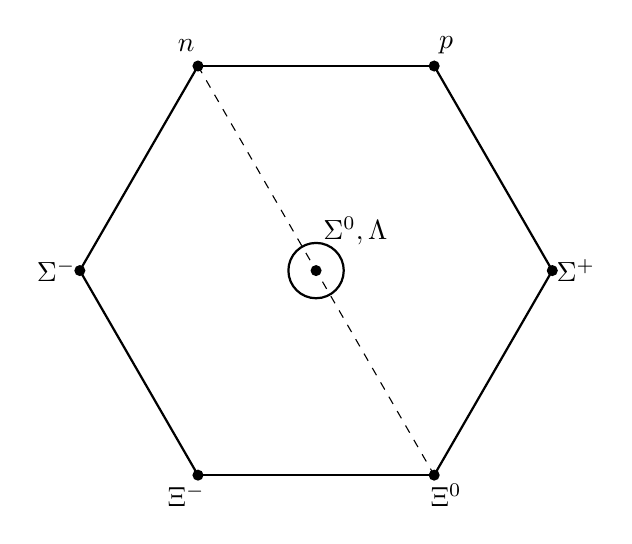
\begin{tikzpicture}

% Segundo hexágono con n en el vértice superior izquierdo y orden en sentido horario
\foreach \angle in {120,60,...,-180} {
  \draw[thick] (\angle:3cm) -- (\angle-60:3cm);
}

% Puntos en los vértices para el segundo hexágono en orden horario con círculos de 2pt
\node at (120:3.3cm) {$n$};
\fill (120:3cm) circle (2pt);

\node at (60:3.3cm) {$p$};
\fill (60:3cm) circle (2pt);

\node at (0:3.3cm) {$\Sigma^+$};
\fill (0:3cm) circle (2pt);

\node at (-60:3.3cm) {$\Xi^0$};
\fill (-60:3cm) circle (2pt);

\node at (-120:3.3cm) {$\Xi^-$};
\fill (-120:3cm) circle (2pt);

\node at (-180:3.3cm) {$\Sigma^-$};
\fill (-180:3cm) circle (2pt);

% Línea diagonal del segundo hexágono
\draw[dashed] (120:3cm) -- (-60:3cm);

% Nombres en el centro
\node at (0.5,0.5) {$\Sigma^0, \Lambda$};
\draw[thick] (0,0) circle (10pt);
\fill[] (0,0) circle (2pt);

\end{tikzpicture}

\end{document}
